% =====================================================================
%  第 4 章 §4.3 几何量子化 —— ch04b（tr05）
%  页段：PDF 151–172（原书 p.141–162）
% =====================================================================
% [原文 p.141]
引理 4.58 表明，黎曼几何中的共轭点是勒让德奇点的一个特殊情形。例如，若 $N$ 是 $M=\R^2$ 中由 $y=x^2$ 表示的子流形，则 $\pi(\varphi_\tau(S^*_N M))$ 如图 4.5 所示，从 $\tau\ge 1/\sqrt2$ 起出现奇点。

\begin{figure}[htbp]
  \centering
  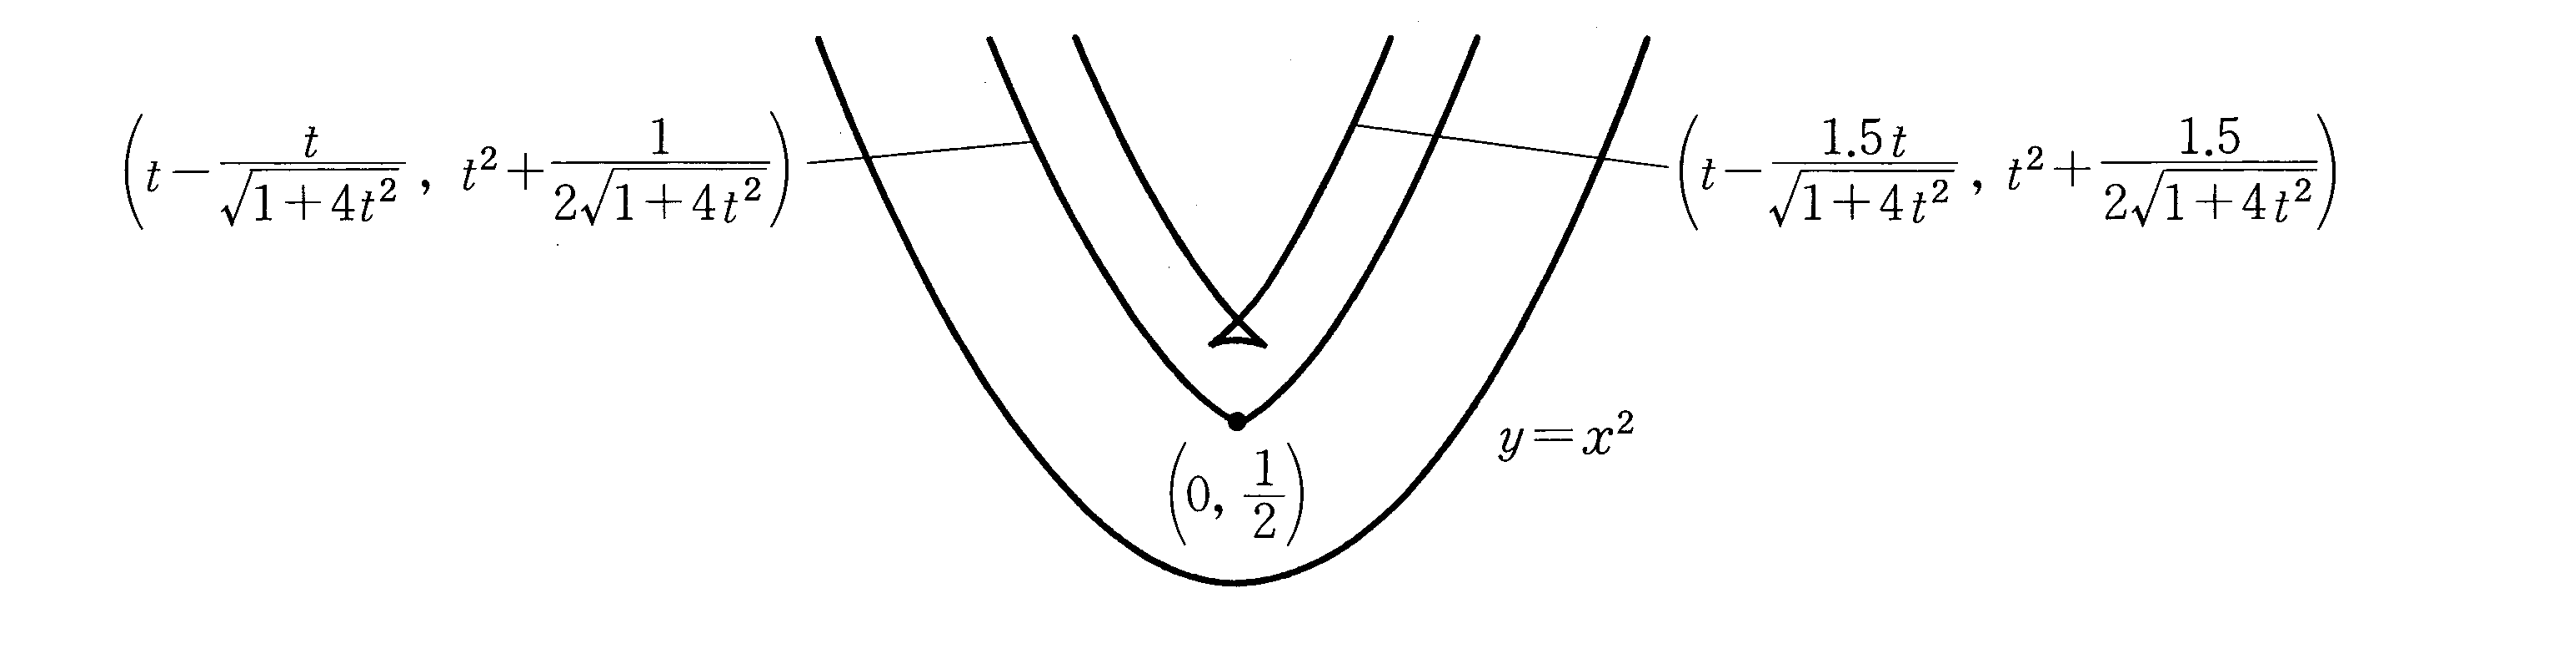
\includegraphics[width=0.95\textwidth]{figures/fig4.5.png}
  \figtitle{4.5}{共轭点（原书 p.141）}
\end{figure}

用几何光学的语言，可以这样看待共轭点。把 $N$ 看作光源，则由 Huygens 原理，时刻 $\tau$ 时光线所能到达范围的边界就是 $\pi(\varphi_\tau(S^*_N M))$。这大概就是“波前”一词的语源。

\section{几何量子化}

\takeaway{拉格朗日纤维丛的纤维与完全可积系统的轨道都是拉格朗日子流形。几何量子化用极化把辛流形化为线丛的截面空间：凯勒极化给出全纯截面，实极化下只有 Bohr–Sommerfeld 轨道上的截面存活。}

本节讲述拉格朗日子流形与完全可积系统、几何量子化的关系。

\begin{lemma*}{4.59}
  对 $\R^n$ 在 $2n$ 维辛流形 $(M,\omega)$ 上保持辛结构的作用，其 $n$ 维轨道是拉格朗日子流形。
\end{lemma*}

\begin{proof}
  设 $T_0\R^n$ 的基元素在 $M$ 上诱导的向量场为 $V_1,\dots,V_n$。则 $[V_i,V_j]=0$。只须证明 $\omega_M(V_i,V_j)=0$。

  局部地考虑，由定理 2.18，存在函数 $f_i$ 使 $V_i=X_{f_i}$（这里 $X_{f_i}$ 是 $f_i$ 决定的哈密顿向量场）。于是
  \begin{equation}
    \omega_M(V_i,V_j)=df_i(V_j)=V_j(f_i)=\{f_i,f_j\} \tag{4.13}
  \end{equation}
  （第 1 个等号是哈密顿向量场的定义，第 2 个等号是外微分的定义，第 3 个等号是泊松括号的定义）。由 $X_{\{f_i,f_j\}}=[V_i,V_j]=0$（定理 2.18）知，(4.13) 为 0。
\end{proof}
% [Tutor Note: 定理 2.18 给出的是“$\alpha$ 闭 $\Leftrightarrow$ 局部为哈密顿向量场”，故 $V_i=X_{f_i}$ 只在局部成立：$\R^n$ 在 $M$ 上的作用一般没有整体的哈密顿函数。结论 $\omega_M(V_i,V_j)=0$ 是逐点性质，局部验证即已足够。]

% [原文 p.142]
\begin{remark}{4.60}
  $\R^n$ 在 $2n+1$ 维接触流形上保持接触形式的作用，其 $2n$ 维轨道是勒让德子流形，这一点也可同样证明。
\end{remark}

回忆完全可积系统的定义。

\begin{definition}{4.61}
  设 $f:M\to\R$ 为 $2n$ 维辛流形 $(M,\omega)$ 上的函数。若哈密顿向量场 $X_f$ 完全可积（complete integrable），是指存在函数 $f_2,\dots,f_n$，使下述条件成立（记 $f=f_1$）：
  (1) $\{f_i,f_j\}=0$。
  (2) $df_1,\dots,df_n$ 在各点线性无关。
\end{definition}

对定义 4.61 的 $f_i$，考虑 $X_{f_i}$ 生成的单参数变换群 $\varphi^i_\tau$，置
\begin{equation}
  (\tau_1,\dots,\tau_n)(p)=\varphi^1_{\tau_1}\circ\cdots\circ\varphi^n_{\tau_n}(p) \tag{4.14}
\end{equation}
由条件 (1) 与定理 2.18，(4.14) 给出 $\R^n$ 在 $M$ 上保持辛结构的作用。进而，由于 $(f_1,\dots,f_n)$ 是动量映射，这个作用是哈密顿作用。由引理 4.59，作用的轨道是拉格朗日子流形。若轨道紧致且可定向，则因它是 $\R^n$ 作用的轨道，轨道成为 $n$ 维环面，而 $X_f$ 在轨道上的限制由 $\R^n$ 上的常系数向量场导出。这叫做 Arnold–Liouville 定理（参看 [13]、[127]）。
% [Tutor Note: 式 (4.14) 的左边 $(\tau_1,\dots,\tau_n)$ 指的是映射 $\R^n\to M$，$\tau_1,\dots,\tau_n$ 应读作该映射在参数 $(\tau_1,\dots,\tau_n)$ 处的像；这不是把 $n$ 个参数当成一个函数的自变量。各 $\varphi^i_{\tau_i}$ 彼此交换，正是条件 (1) 中 $\{f_i,f_j\}=0$ 的积分形式。]

把群作用稍作推广，来考虑纤维丛的结构与叶状结构。

\begin{definition}{4.62}
  纤维丛 $\pi:M\to N$ 为拉格朗日纤维丛（Lagrangian fibration），是指它的每个纤维都是拉格朗日子流形。

  $M$ 上的叶状结构为拉格朗日叶状结构（Lagrangian foliation），是指它的每个叶都是拉格朗日子流形。
\end{definition}

叶状结构的定义参看 [355] 等。

\begin{theorem*}{4.63}
  设 $\pi:M\to N$ 为纤维紧致、连通且可定向的拉格朗日纤维丛。
  (1) 纤维同胚于环面 $T^n$。

% [原文 p.143]
  (2) 对任意 $p_0\in N$，存在 $p_0$ 的邻域 $U$ 与 $\pi^{-1}(U)$ 上 $T^n$ 的作用，使 $T^n$ 的轨道恰为 $\pi$ 的纤维。
  (3) 存在微分同胚 $\bar f:U\to\bar f(U)\subset\R^n$，使 $f=\bar f\circ\pi$ 是 $T^n$ 作用的动量映射。
\end{theorem*}

\begin{proof}
  必要时把 $N$ 取小，不妨设 $N\subset\R^n$。设 $f'_i:M\to\R$ 为 $\pi:M\to N\subset\R^n$ 与第 $i$ 个坐标函数的复合。取 $x\in M$，$p=\pi(x)\in N$，$V\in T_x(\pi^{-1}(p))$。因 $df'_i(V)=V(f'_i)=0$，由定义得 $\omega(X_{f'_i},V)=df'_i(V)=0$。由于 $\pi^{-1}(p)$ 是拉格朗日子流形，可知 $X_{f'_i}\in T_x(\pi^{-1}(p))$。也就是说 $X_{f'_i}f'_j=0$。换言之，$\{f'_i,f'_j\}=0$。于是诸 $X_{f'_i}$ 生成 $\R^n$ 的作用，而 $\pi$ 的纤维就是它的轨道。由 Arnold–Liouville 定理，得到 (1)。

  替换 $f'_i$，来构造 $f=(f_1,\dots,f_n):N\to\R^n$。取 $\gamma_i:S^1\to T^n$（$i=1,\dots,n$）为 $H_1(\pi^{-1}(p_0);\Z)$ 的生成元。当 $p$ 接近 $p_0$ 时，可以把 $\pi^{-1}(p)$ 的闭曲线 $\gamma^p_i$ 取在 $\gamma_i$ 附近。取 $\psi^p_i:[0,1]\times S^1\to M$，使 $\psi^p_i(0,t)=\gamma_i(t)$，$\psi^p_i(1,t)=\gamma^p_i(t)$（图 4.6）。置 $\bar f_i(p)=\int\psi^{*p}_i\omega_M$。由于 $\pi$ 的纤维是拉格朗日子流形，$f_i(p)$ 只依赖于 $\gamma_i$ 的同调类与 $p$，而不依赖于 $\gamma_i$、$\psi^p_i$。
% [Tutor Note: 原书 p.143 此句作 $f_i(p)$，与上一句刚定义的 $\bar f_i(p)$ 不符；此处 $f_i$ 应即定义在 $N$ 上的 $\bar f_i$（下文 $f_i=\bar f_i\circ\pi$），疑为原书漏排上划线，正文照录。]
\end{proof}

\begin{lemma*}{4.64}
  $d\bar f_1\wedge\cdots\wedge d\bar f_n\ne 0$。
\end{lemma*}

\begin{proof}
  取微分同胚 $\varphi:(S^1)^n\to T^n=\pi^{-1}(p_0)$，使 $\varphi_*$ 把第 $i$ 个 $[S^1]$ 移到 $[\gamma_i]$。可以取到映入像中的微分同胚 $\bar\varphi:(S^1)^n\times V\to M$，使 $\bar\varphi$ 把 $(S^1)^n\times\{1\text{ 点}\}$ 映为 $\pi$ 的纤维。不妨设 $V\subset\R^n$，$p_0=0$。于是由定义，对 $p=(p_1,\dots,p_n)\in V$ 有
  \[
    \int_{(S^1)^n\times[0,p_1]\times\cdots\times[0,p_n]}\bar\varphi^*\omega^n
    =(-1)^n\bar f_1(p_1)\cdots\bar f_n(p_n)
  \]
  容易看出。由于 $\bar\varphi^*\omega^n$ 是体积元素，引理得证。
\end{proof}

考虑以 $f=(f_1,\dots,f_n)$、$f_i=\bar f_i\circ\pi$ 为动量映射的 $\R^n$ 作用。由引理 4.64，其轨道与 $\pi$ 的纤维一致。设 $\exp(tX_{f_i})$ 为哈密顿向量场 $X_{f_i}$ 生成的单参数变换群。

\begin{lemma*}{4.65}
  对任意 $x\in M$，$\exp(X_{f_i})(x)=x$。即 $\exp(tX_{f_i})$ 具有周期 1。
\end{lemma*}

% [原文 p.144]
\begin{figure}[htbp]
  \centering
  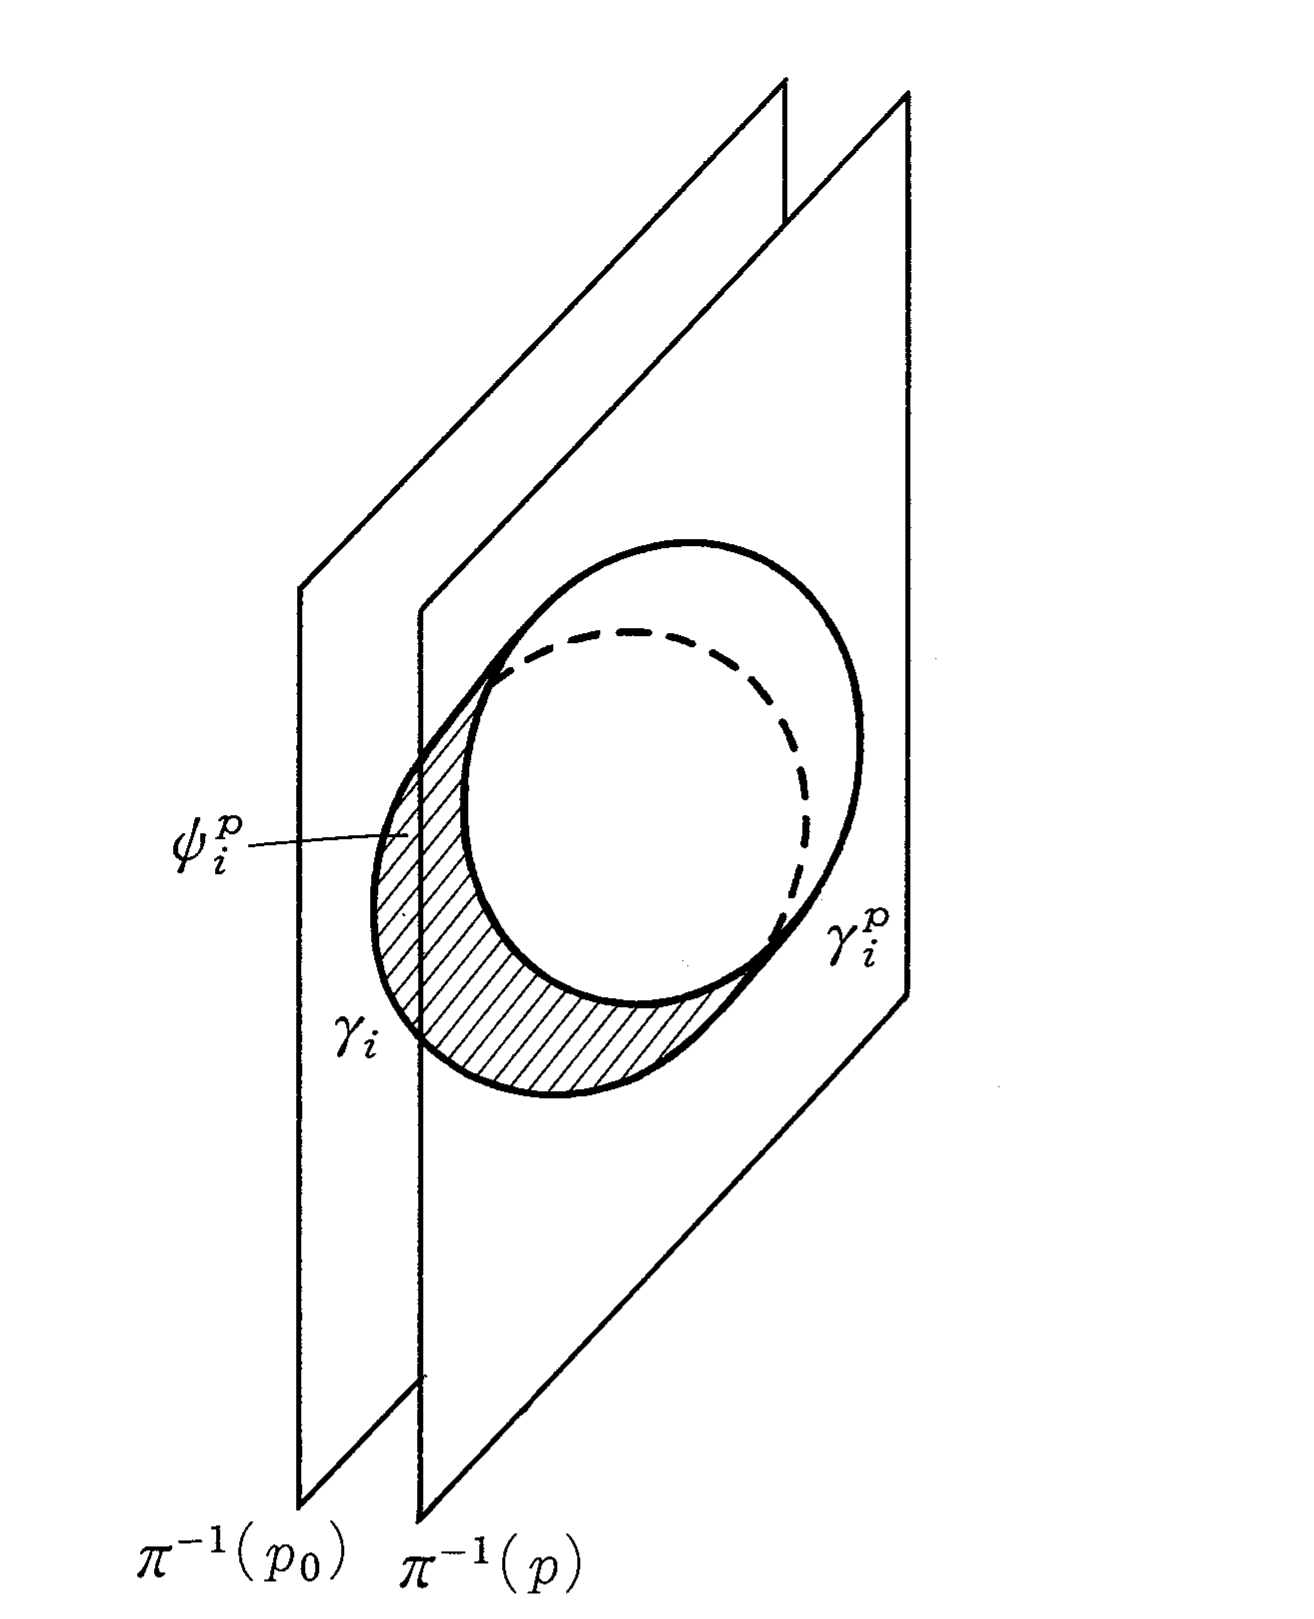
\includegraphics[height=0.34\textheight]{figures/fig4.6.png}
  \figtitle{4.6}{角-动量坐标的作法（原书 p.144）}
\end{figure}

\begin{proof}
  不妨设 $\pi(x)=p_0$。由 Arnold–Liouville 定理，存在线性无关的向量 $\vec t_1,\dots,\vec t_n\in\R^n$（$\vec t_i=(t_{i,1},\dots,t_{i,n})$），使
  \[
    \exp(t_{i,1}X_{f_1}+\cdots+t_{i,n}X_{f_n})(x)=x
  \]
  成立。置 $\ell_i$ 为闭曲线 $\tau\mapsto\exp(\tau(t_{i,1}X_{f_1}+\cdots+t_{i,n}X_{f_n}))(x)$。不妨设 $\ell_i$ 是 $H_1(\pi^{-1}(p_0);\Z)$ 的生成元。设 $\ell^p_i$ 为 $\pi^{-1}(p)$ 中在 $\ell_i$ 附近的闭曲线，设 $\phi^p_i:[0,1]\times S^1\to M$ 为以 $\ell_i$ 与 $\ell^p_i$ 为边界的映射（图 4.6）。则
  \[
    \int\phi_i^*\omega_M=\sum t_{i,j}\bar f_j(p)
  \]
  另一方面，设 $[\ell_i]=\sum n_{i,j}[\gamma_j]$，则
  \[
    \int\phi_i^*\omega_M=\sum n_{i,j}\bar f_j(p)
  \]
  所以 $t_{i,j}=n_{i,j}$ 为整数，把 $i,j$ 变动而看作矩阵时它是 $SL(n;\Z)$ 的元素。引理由此得到。
\end{proof}
% [Tutor Note: 原书 p.144 把这里的同伦写成 $\phi^p_i$，而 p.143 定义它时写作 $\psi^p_i$，两处指同一族以 $\ell_i$、$\ell^p_i$（或 $\gamma_i$、$\gamma^p_i$）为边界的映射，只是记号换了字母。]

至此，定理 4.63 的证明完成。

考察定理 4.63 的 $f=(f_1,\dots,f_n)$。选取截面 $s:U\to M$，定义 $\varphi:T^n\times\bar f(U)\to M$ 为下式：
% [原文 p.145]
\begin{equation}
  \varphi(\vec t,\vec p)=\vec t\cdot s(\bar f^{-1}(\vec p)). \tag{4.15}
\end{equation}

\begin{definition}{4.66}
  (4.15) 称为角-动量坐标（action angle coordinate）。
\end{definition}

举几个拉格朗日纤维丛的例子。

\begin{example}{4.67}
  余切丛 $T^*N\to N$ 是拉格朗日纤维丛。
\end{example}

\begin{example}{4.68}
  \begin{equation}
    N_1=\left\{\begin{pmatrix}1&p_1&q_2\\0&1&p_2\\0&0&1\end{pmatrix}\ \middle|\ p_1,p_2,q_2\in\R\right\} \tag{4.16}
  \end{equation}
  \begin{equation}
    N_2=\left\{\begin{pmatrix}1&q_1\\0&1\end{pmatrix}\ \middle|\ q_1\in\R\right\} \tag{4.17}
  \end{equation}
  设 $N_1$、$N_2$ 如上。又把其中 $p_i,q_i\in\Z$ 的情形分别写作 $\Gamma_1,\Gamma_2$。置 $M=N_1/\Gamma_1\times N_2/\Gamma_2$。$dq_1\wedge dp_1+dq_2\wedge dp_2$ 是 $N_1\times N_2$ 上的闭 2 形式，且在 $\Gamma_1\times\Gamma_2$ 下不变。因此，$M$ 上确定了一个 2 形式 $\omega_M$。$\omega_M$ 确定辛结构是显然的。

  由于 $H_1(M;\Z)=\Z^3$，$M$ 不能成为凯勒流形\footnote{这个例子，研究复曲面分类的学者在 1950、60 年代（小平等人）大概就已知道。后来（1970 年前后）Thurstone 也注意到了这一点。}。（由 Hodge 理论可知，凯勒流形的奇数阶 Betti 数是偶数。）

  $[q_1,q_2,p_1,p_2]\mapsto[p_1,p_2]$ 确定 $M\to T^2$ 这一拉格朗日纤维丛。
\end{example}

\begin{example}{4.69}
  考虑环面流形 $M$，置动量映射 $f:M\to\R^n$ 的临界值集合为 $X\subset\R^n$。$f$ 在 $M-f^{-1}(X)$ 上的限制给出以 $\R^n-X$ 的连通分支为底空间的拉格朗日纤维丛。
\end{example}

\begin{example}{4.70}
  设 $M$ 为 K3 曲面。K3 曲面上存在 Ricci 曲率为 0 的黎曼度量（Calabi–Yau 度量）$g_M$。此外，存在 3 种复结构 $I,J,K$，满足 $I^2=J^2=K^2=-1$，$IJ=K$，并且由 $I,J,K$ 得到辛结构 $\omega_I,\omega_J,\omega_K$，使 $(M,g_M,I,\omega_I)$、$(M,g_M,J,\omega_J)$、

% [原文 p.146]
  $(M,g_M,K,\omega_K)$ 都成为凯勒流形。（以上事实称为 K3 曲面是超凯勒流形（hyper Kähler 流形）。以上事实的证明参看 [281]。）

  若适当选取 $g_M$ 与 $I$，则已知存在全纯映射 $\pi:(M,I)\to\CP^1$（椭圆型 K3 曲面）。

  设 $\pi(x)=p$，$V\in T_x\pi^{-1}(p)$。则 $I(V)\in T_x\pi^{-1}(p)$，且 $V,I(V)$ 是 $T_x\pi^{-1}(p)$ 的基。又 $V,I(V),J(V),K(V)$ 互相正交。因此 $\omega_J(V,I(V))=g_M(V,JI(V))=0$。也就是说，$\pi$ 的纤维关于辛结构 $\omega_J$ 是拉格朗日子流形。（不过 $\pi$ 有奇异纤维，并非拉格朗日纤维丛。）
\end{example}
% [Tutor Note: $I(V)\in T_x\pi^{-1}(p)$ 用到了 $\pi$ 关于 $I$ 全纯：全纯映射的纤维是复子流形，故切空间对 $I$ 不变。两两正交则来自超凯勒结构 $I^2=J^2=K^2=-1$、$IJ=K$ 与 $g_M$ 关于三者的 Hermite 性。]

\begin{remark}{4.71}
  如例 4.69、4.70 所示，在拉格朗日纤维丛的定义中要求它是纤维丛，换言之要求各点的纤维全都相同，这在许多情形下是过强的假设。在例外集合上允许出现奇异纤维，看来才是自然的。可积系统的定义恐怕也一样。
\end{remark}

如 §6.6 所见，拉格朗日纤维丛在镜像对称中起重要作用。

与拉格朗日纤维丛关系密切的话题是几何量子化。几何量子化始于 Kostant [223]、Souriau [345]。详细解说见 [34]、[196]、[199]、[344]、[354]、[399] 等。

回忆第 1 章所述的问题 1.5。问题 1.5 说的是：对辛流形 $M$ 构造 Hilbert 空间 $\cH$，并对 $C^\infty(M)$ 的元素构造算子 $\cH\to\cH$。其中一半即 $\cH$ 的构造，称为预量子化（prequantization）。$\cH$ 的构造的范本是 $M$ 为余切丛 $T^*N$ 的情形，此时 $\cH=L^2(N)$。是 $L^2(N)$ 而不是 $L^2(T^*N)$。也就是说，它不是辛流形上的函数空间，而是维数为其一半的空间 $N$ 上的函数空间。这种把函数空间劈成一半的操作，就是预量子化。

一般的辛流形的情形，为构造预量子化，需

% [原文 p.147]
要用极化这一概念。

\begin{definition}{4.72}
  辛流形 $(M,\omega_M)$ 的极化（polarization），是指 $TM\otimes\C$ 的秩 $n$ 复子向量丛 $P$，满足下列条件者。
  (1) 若 $V,W$ 是 $P$ 的截面，则 $[V,W]$（向量场的交换子）也是 $P$ 的截面。
  (2) 若 $V,W$ 是 $P$ 的截面，则 $\omega_M(V,W)=0$（这里把 $\omega_M$ 按复双线性延拓到 $TM\otimes\C$ 上）。
\end{definition}

\begin{example}{4.73}
  设 $(M,J_M,\omega_M)$ 为凯勒流形。把 $TM\otimes\C$ 分解为 $TM\otimes\C=T^{1,0}M\oplus T^{0,1}M$（式 (2.15)）。置 $P=T^{0,1}M$。由于 $J_M$ 可积，条件 (1) 成立（引理 2.34）。又若 $V,W\in\Gamma(T^{0,1}M)$，则
  \[
    \omega_M(V,W)=\omega_M(J_MV,J_MW)=\omega_M(\sqrt{-1}V,\sqrt{-1}W)=-\omega_M(V,W)
  \]
  因此 (2) 成立。这个 $P$ 称为凯勒极化（Kähler polarization）。
\end{example}

\begin{example}{4.74}
  设 $\pi:M\to N$ 为拉格朗日纤维丛。置 $P_x$ 为纤维方向的切空间全体，即 $P_x=T_x(\pi^{-1}(x))\otimes\C$，则 (1)、(2) 均被满足。这个极化称为实极化（real polarization）。即使不从拉格朗日纤维丛、而从拉格朗日叶状结构出发，也同样可以定义极化。
\end{example}

考虑余切丛 $T^*N\to N$ 的实极化 $P$，置
\begin{equation}
  \cH_0=\{s\in C^\infty(T^*N)\mid \forall V\in\Gamma(P),\ Vs=0\} \tag{4.18}
\end{equation}
（以下本节中，$C^\infty(M)$ 等均指光滑复值函数的集合。）由定义，$\cH_0$ 是纤维上取常值的 $T^*M$ 上的函数全体，也就是 $M$ 上的函数全体。因此，其完备化就是 $\cH$。
% [Tutor Note: 本段开头说的是余切丛 $T^*N\to N$，此处却写成 $T^*M$ 与 $M$；按上下文这两处应分别读作 $T^*N$ 与 $N$。原书如此，未改。]

余切丛以外的 $M$ 与其上的极化 $P$ 的情形，(4.18) 可以推广。然而为此不能只考虑函数，必须考虑线丛的截面。设 $(\cL,\nabla)$ 为定义 4.30 的预量子化丛。

% [原文 p.148]
\begin{remark}{4.75}
  当 $[\omega_M]$ 不是整系数上同调类时，预量子化丛不存在。$[\omega_M]$ 不是整系数上同调类时如何考虑预量子化，我想是个有趣的问题。
\end{remark}

\begin{definition}{4.76}
  $\cH_0(M,\omega_M,P)=\{s\in\Gamma(M;\cL)\mid \forall V\in\Gamma(P),\ \nabla_Vs=0\}$。
\end{definition}

这是暂定的定义。之所以说是暂定的，理由后述。

首先考虑凯勒极化的情形。此时定义 4.76 行得通。设 $(M,\omega_M,g_M)$ 为凯勒流形，把 $\nabla:\Gamma(M;\cL)\to\Gamma(M;\cL\otimes\Lambda M)$ 分解为 $\nabla=\nabla^{1,0}+\nabla^{0,1}$。这里 $\nabla^{1,0}:\Gamma(M;\cL)\to\Gamma(M;\cL\otimes\Lambda^{1,0}M)$，$\nabla^{0,1}:\Gamma(M;\cL)\to\Gamma(M;\cL\otimes\Lambda^{0,1}M)$。

\begin{lemma*}{4.77}
  置 $\bar\partial=\nabla^{0,1}$，则 $\bar\partial$ 确定 $\cL$ 的复结构。
\end{lemma*}

\begin{proof}
  由于 $\omega\in\Lambda^{1,1}M$ 且 $\nabla^2=2\pi\sqrt{-1}\omega\wedge$，故 $\bar\partial^2=0$。于是由定理 2.49，引理得证。
\end{proof}

由引理 4.77 可知下面的事实。

\begin{lemma*}{4.78}
  在凯勒极化 $P$ 的情形，$\cH_0(M,\omega_M,P)$ 与 $\cL$ 的全纯截面全体一致。
\end{lemma*}

\begin{proof}
  “对任意 $V\in\Gamma(P)$ 都有 $\nabla_Vs=0$”这一条件与 $\bar\partial s=0$ 等价。
\end{proof}

下面考虑实极化的情形。为此，来证明与命题 4.51 类似的引理 4.79。设 $(M,\omega_M)$ 为辛流形，$(\cL,\nabla)$ 为预量子化丛。设 $L$ 为 $M$ 的拉格朗日子流形，则 $F_\nabla=2\pi\sqrt{-1}\omega$，故 $(\cL,\nabla)$ 在 $L$ 上的限制是平坦向量丛。考虑接触流形 $(S(\cL),\theta)$。

\begin{lemma*}{4.79}
  下述两个条件等价。
  (1) 存在勒让德子流形 $\tilde L\subset S(\cL)$，使 $\pi(\tilde L)=L$，且 $\pi$ 在 $\tilde L$ 上单射。
  (2) $(\cL,\nabla)$ 在 $L$ 上的限制是平凡的。
\end{lemma*}

\begin{proof}
  对截面 $s:L\to S(\cL)$，“$s(L)$ 是勒让德子流形”这一条件与“$s$ 关于联络 $\nabla$ 平行（$\nabla s=0$）”这一条件

% [原文 p.149]
  等价。由此引理得证。
\end{proof}

\begin{definition}{4.80}
  称 $L$ 为 Bohr–Sommerfeld 轨道（Bohr–Sommerfeld orbit），是指引理 4.79 的等价条件被满足。
\end{definition}

设 $\pi:M\to N$ 为拉格朗日纤维丛，$(\cL,\nabla)$ 为预量子化丛。

\begin{lemma*}{4.81}
  若 $M$ 紧致，则 $\pi:M\to N$ 的纤维中是 Bohr–Sommerfeld 轨道的只有有限个。
\end{lemma*}

\begin{proof}
  设 $T^n(p)=\pi^{-1}(p_0)$ 为 Bohr–Sommerfeld 轨道。只须证明：对接近 $p_0$ 的 $p$，$T^n(p)$ 不是 Bohr–Sommerfeld 轨道。
% [Tutor Note: 原书 p.149 此处印作 $T^n(p)=\pi^{-1}(p_0)$，据上下文应读作 $T^n(p)=\pi^{-1}(p)$、并把语句中的 $p$ 读作 $p_0$；正文照录原书。]

  取 $\gamma_1,\dots,\gamma_n$ 为 $H_1(T^n(p_0);\Z)$ 的基。当 $p$ 是接近 $p_0$ 的点时，可把 $\gamma_i$ 看作 $H_1(T^n(p);\Z)$ 的元素。把这个基 $\gamma_i$ 写作 $\gamma^p_i$。对 $p$ 置 $h_i(p)=\log\operatorname{hol}_{\gamma^p_i}\nabla$。也就是说，$h_i(p)$ 是联络 $\nabla$ 沿道路 $\gamma^p_i$ 的和乐 $\operatorname{hol}_{\gamma^p_i}\nabla$ 的对数（$\log$ 取在 $p_0$ 处为 0 的分支）。只须证明 $dh_i$（$i=1,\dots,n$）线性无关。

  考虑定理 4.63 的动量映射 $f:\pi^{-1}(U)\to\R^n$。与定理 4.63 的证明同样地取 $\psi^p_i:[0,1]\times S^1\to M$，即 $\psi^p_i(0,t)=\gamma^{p_0}_i(t)$，$\psi^p_i(1,t)=\gamma^p_i(t)$（图 4.6）。由于 $F_\nabla=2\pi\sqrt{-1}\omega$，由和乐与曲率之间熟知的关系式，
  \begin{equation}
    h_i(p)=2\pi\sqrt{-1}\int_{[0,1]\times S^1}\psi^{p*}_i\omega \tag{4.19}
  \end{equation}
  又由 (4.19) 与 $f_i$ 的定义，
  \begin{equation}
    h_i(p)=2\pi\sqrt{-1}f_i(p) \tag{4.20}
  \end{equation}
  也就是说，$dh_i$（$i=1,\dots,n$）线性无关。
\end{proof}

用引理 4.81 证明中的计算，可以证明下述定理。

\begin{theorem*}{4.82}
  设 $(M,\omega_M)$ 上有哈密顿环面作用，$f:M\to\R^n$ 为动量映射。设 $f^{-1}(0)$ 是 Bohr–Sommerfeld 轨道。当 $f^{-1}(p)$ 为 $n$ 维时，下述两者等价。
  (1) $f^{-1}(p)$ 是 Bohr–Sommerfeld 轨道。
  (2) $p\in\Z^n$。
\end{theorem*}

\begin{proof}
  由 (4.20)，沿 $\gamma^p_i\in H_1(f^{-1}(p);\Z)$ 的 $\nabla$ 的和乐是，

% [原文 p.150]
  $\exp(2\pi\sqrt{-1}f_i(p))$。由此定理得证。
\end{proof}

现在，把定义 4.76 套用到由拉格朗日纤维丛 $\pi:M\to N$ 得到的实极化的情形试试看。设对 $\cL$ 的光滑截面 $s$，$\nabla_Vs=0$ 对 $V\in P$ 成立。那么，$s$ 在纤维 $f^{-1}(p)$ 上的限制就满足 $\nabla s=0$（因为 $P$ 是纤维方向的向量场全体）。因此，只要 $\cL$ 在 $f^{-1}(p)$ 上不平凡（也就是说，只要 $f^{-1}(p)$ 不是 Bohr–Sommerfeld 轨道），$s$ 在纤维 $f^{-1}(p)$ 上的限制就是 0。于是由引理 4.81，$s$ 必须为 0。结果得到 $\cH_0(M,\omega,P)=0$。这就是把定义 4.76 说成暂定的理由。

为修正这一点，把“只在 Bohr–Sommerfeld 轨道上不为 0，且在 Bohr–Sommerfeld 轨道上关于 $\nabla$ 平行”这样的超函数式截面承认为 $\cH$ 的元素，大概是恰当的。于是如下定义。

\begin{definition}{4.83}
  设使 $f^{-1}(p)$ 为 Bohr–Sommerfeld 轨道的 $p$ 的个数为 $\ell$，则定义前量子化 $\cH(M,\omega_M,P)$ 为 $\C^\ell$。
\end{definition}

\begin{remark}{4.84}
  例 4.69 的情形（环面流形）有奇异纤维，定义 4.83 不能照搬。此时参看定理 4.82，如下定义。

  设 $f:M\to\R^n$ 为动量映射，$\ell$ 为 $f(M)\cap\Z^n$ 的点的个数。此时，前量子化 $\cH(M,\omega_M,P)$ 为 $\C^\ell$。（注意这个定义把退化的“Bohr–Sommerfeld 轨道”也计算在内。）
\end{remark}

\begin{remark}{4.85}
  Bohr–Sommerfeld 量子条件是这样的。考虑由能量（哈密顿函数）不超过一定值 $E_0$ 的不等式给出的相空间（辛流形）的紧致子集，数其中所含哈密顿向量场的轨道里满足某个整数性条件（量子条件）的轨道个数。这个数，与量子力学中能量不超过 $E_0$ 的状态空间的维数一致\footnote{§4.4 讨论的 Maslov 指数，是作为对 Bohr–Sommerfeld 量子条件的修正而被发现的。参看 [246]、[34]、[165]。}。
\end{remark}
% [Tutor Note: 这里“量子化后的 Hilbert 空间维数 = 满足量子条件的轨道数”正是 Bohr–Sommerfeld 旧量子论的对应原理；$\ell$ 有限是引理 4.81 的结论。定义 4.83 用 $\C^\ell$ 而不是 $L^2$，是因为实极化的正则截面只能分布在有限条 BS 轨道上。]

% [原文 p.151]
把“哈密顿向量场的轨道”换成拉格朗日纤维丛的纤维，把“某个整数性条件”换成 Bohr–Sommerfeld 轨道这一条件，则由实极化的预量子化得到的 Hilbert 空间正对应于量子力学的状态空间。

量子力学情形的另一种表述，即属于 $E_0$ 以下特征值的特征向量个数的类似物，大概是凯勒极化。

\begin{remark}{4.86}
  把层 $\cF_P$ 定义为前层
  \[
    \cF_P(U)=\{s\mid s\in\Gamma(U,\cL),\ \nabla s=0\}
  \]
  的层化。此时，对定义 4.72 的 $\cH(M,\omega_M,P)$，$\bigoplus H^*(M;\cF_P)\cong\cH(M,\omega_M,P)$ 已由 Śniatycki [343] 证明。
\end{remark}
% [Tutor Note: 原书 p.151 写作“定义 4.72 的 $\cH(M,\omega_M,P)$”，但 4.72 只定义极化；$\cH(M,\omega_M,P)$ 是在定义 4.76、4.83 中定义的，引用编号疑有误，正文照录。]

环面流形的情形，由实极化与凯勒极化得到的前量子化彼此一致。这一事实在环面流形的代数几何中大概已为人知，但注意到它与几何量子化之关系的，我想是 Guillemin–Sternberg [168]。

\begin{theorem}{4.87}
  对环面流形 $(M,J_M,\omega_M)$，
  \[
    \rank H^0(M;\cL)=\#(f(M)\cap\Z^n)
  \]
  成立。这里 $\cL$ 是前量子化丛，$f:M\to\R^n$ 是动量映射。
\end{theorem}

\begin{remark}{4.88}
  把辛形式 $\omega_M$ 乘以正整数 $m$，前量子化丛 $\cL$ 就换成 $\cL^{\otimes m}$。另一方面动量映射 $f$ 变为 $mf$。于是 $\#(mf(M)\cap\Z^n)$ 渐近地接近 $f(M)$ 的体积的 $m^n$ 倍。因此由定理 4.87，
  \begin{equation}
    \lim_{m\to\infty}\frac{\rank H^0(M;\cL^{\otimes m})}{m^n\vol(f(M))}=1 \tag{4.21}
  \end{equation}
  可知。研究 $\rank H^0(M;\cL^{\otimes m})$ 在 $m\to\infty$ 时的行为，在代数几何中是重要的。
\end{remark}

\begin{remark}{4.89}
  $\cH(M,\omega_M,P_M)$ 本应是 Hilbert 空间，故必须定义内积。又对两个互不相同的极化 $P_1,P_2$，$\cH(M,\omega_M,P_1)$、$\cH(M,\omega_M,P_2)$ 之间的配对 $\cH(M,\omega_M,P_1)\otimes\cH(M,\omega_M,P_2)\to\C$ 也在种种情形下已构造出来，称为 Blatter–Kostant–Sternberg 对合（BKS pairing）。这是重要的话题，但本书不讨论。参看 [199]、[344]、[354] 等。
\end{remark}

% [原文 p.152]
几何量子化的下一阶段，是由 $M$ 上的函数构造 $\cH(M,\omega_M,P_M)$ 上的算子。这大概与 $M$ 上函数所成环的环结构的形变（形变量子化等）也有关联，但这一方向的研究看来还处于初期阶段。

下面讨论辛商与几何量子化的关系。为此，先定义动量映射的概念在接触流形中的类似物。

设紧致 Lie 群 $G$ 为 $\Aut(M,\xi_M)$ 的子群，$\xi_M=\Ker\theta_M$。把 $\theta_M$ 换成它关于 $G$ 作用的平均，就能使 $g^*\theta_M=\theta_M$ 对任意 $g\in G$ 成立。以下假定如此。

\begin{definition}{4.90}
  $f:M\to\mathfrak{g}^*$ 是动量映射，是指下列 (1)、(2) 成立。
  (1) 对任意 $W\in\mathfrak{g}$ 与 $N$ 上的任意向量场 $V$，有 $(df)(V)(W)=(d\theta_M)(W,V)$，且 $(\theta_M)(W)(p)=f(p)(W)$。
  (2) $f(g\cdot p)=(\operatorname{ad}g)f(p)$。
\end{definition}
% [Tutor Note: 原书 p.152 的 (1) 写作“$N$ 上的任意向量场 $V$”，而本节讨论的是接触流形 $M$（$N$ 是上一节拉格朗日纤维丛的底空间），此处应读作 $M$；正文照录原书。]

\begin{remark}{4.91}
  定义 4.90(1) 要求 $(df)(V)(W)=(d\theta_M)(W,V)$ 对任意 $V$ 成立。这乍看是“$f_W(p)=f(p)(W)$ 所生成的哈密顿向量场为 $W$”这一条件，比定义 4.22(1) 强。但是，由于我们假定了 $g^*\theta_M=\theta_M$，由引理 4.26(2)，$X_{-1}(f_W)=L_W\theta_M=0$。也就是说，$(df)(X_{-1})(W)=0=(d\theta_M)(W,X_{-1})$ 自动成立。因此，定义 4.90(1) 与“$f_W$ 所生成的哈密顿向量场为 $W$”这一条件等价。
\end{remark}

下述定理是定理 3.2 的类似，证明也相同。

\begin{theorem}{4.92}
  动量映射 $f:M\to\mathfrak{g}^*$ 总是存在。
\end{theorem}

\begin{remark}{4.93}
  辛流形情形的定理 3.2 需要 $H^1(M;\R)=0$ 这一假定。接触流形情形则不需要。回想一下：保持接触结构的任意向量场都是哈密顿向量场（定理 4.28）。
\end{remark}

当 $\cL\to M$ 为预量子化丛时，保持辛结构的 $M$ 的向量场 $V$ 能提升为 $S(\cL)$ 上保持接触结构的向量场，其充要条件是：$V$ 为哈密顿向量场。

% [原文 p.153]
下面设 $\cL\to M$ 为辛流形 $M$ 的预量子化丛。设紧致 Lie 群 $G$ 在 $M$ 上有哈密顿作用，动量映射为 $f:M\to\mathfrak{g}^*$。构造辛商 $\quot{M}{G}$ 的预量子化丛，是以下一段的目标。

用 $f\circ\pi:S(\cL)\to\mathfrak{g}^*$，如下确定 $i:\mathfrak{g}\to\operatorname{Lie}(S(\cL))$。取 $v\in\mathfrak{g}$。考虑函数 $f_v(x)=f(\pi(x))(v):S(\cL)\to\R$，把它的哈密顿向量场 $X_{f_v}$ 记为 $i(v)$。把 $\partial/\partial t$ 记为 $S(\cL)$ 的 Reeb 向量场，即纤维方向的向量场。

\begin{lemma*}{4.94}
  \[
    [i(v),i(w)]=i[v,w]+\omega_M(v,w)(p)\frac{\partial}{\partial t}
  \]
  成立。右边第 2 项中把 $v,w$ 看作 $M$ 上的向量场。
\end{lemma*}

\begin{proof}
  $p\mapsto f(p)(v)$ 所生成的哈密顿向量场与 $v$ 在 $M$ 上诱导的向量场一致，这正是动量映射的定义本身。因此，把 $[i(v),i(w)]$ 投影到底空间，就得到 $i[v,w]$。

  下面考察纤维方向的成分。设 $\theta$ 为 $S(\cL)$ 的接触形式。由定义，$\theta(X_{f_v})=\theta(X_{f_w})=0$。又 $\theta$ 是联络形式，故 $X_{f_v},X_{f_w}$ 是 $v,w$ 的水平提升（horizontal lift）。于是由曲率的定义，
  \[
    2\pi\sqrt{-1}[X_{f_v},X_{f_w}]=F_\nabla(v,w)\frac{\partial}{\partial t}
  \]
  成立。由于曲率 $F_\nabla$ 与 $2\pi\sqrt{-1}\omega_M$ 一致，引理得证。
\end{proof}

\begin{example}{4.95}
  设 $M=\C^2$，$G=U(2)$，考虑 $G$ 在 $M$ 上的线性作用。置
  \[
    v=\begin{pmatrix}0&1\\-1&0\end{pmatrix}\in u(2),\qquad
    w=\begin{pmatrix}0&\sqrt{-1}\\\sqrt{-1}&0\end{pmatrix}\in u(2),
  \]
  则 $\omega_{\C^2}(v,w)(1,0)\ne 0$。
\end{example}

\begin{remark}{4.96}
  引理 4.94 表明，$\mathfrak{g}$ 的作用不能提升到 $S(\cL)$，而 $\mathfrak{g}$ 的中心扩张 $\hat{\mathfrak{g}}$

% [原文 p.154]
  的作用能提升。也就是说，存在正合列
  \[
    1\to\R\to\hat{\mathfrak{g}}\to\mathfrak{g}\to 1
  \]
  且 $\R$ 与 $\hat{\mathfrak{g}}$ 的所有元素交换。

  当古典的某系统具有由某个 Lie 环 $\mathfrak{g}$ 表示的对称性时，量子化后的系统的对称性往往由取中心扩张后的 Lie 环表示。引理 4.94 是其根据之一。参看 [148]。
\end{remark}

\begin{lemma*}{4.97}
  若 $f(p)=0$，则 $\omega_M(v,w)(p)=0$。
\end{lemma*}

\begin{proof}
  由动量映射的定义，$\omega_M(v,w)(p)=-(d_pf)(v)(w)$；而 $f^{-1}(0)$ 在 $G$ 下不变，故 $(d_pf)(v)=0$。
\end{proof}

由引理 4.97，$\mathfrak{g}$ 的作用提升到 $(\pi\circ f)^{-1}(0)\subset S(\cL)$ 上。要提升 Lie 群的作用，还需要另一个条件。为简单起见，设 $M$ 连通。

\begin{lemma*}{4.98}
  设 $p\in f^{-1}(0)$，$G\cdot p$ 为 $G$ 的轨道。
  (1) $\cL$ 在 $G\cdot p$ 上的限制确定 $G\sim G\cdot p$ 上的平坦向量丛 $\cL|_G$。
  (2) $\cL|_G$ 不依赖于 $p$ 的取法。
  (3) $\cL|_G$ 平凡，与“Lie 环 $\mathfrak{g}$ 在 $(\pi\circ f)^{-1}(0)$ 上的作用诱导 Lie 群 $G$ 在 $f^{-1}(0)$ 上的作用”等价。
\end{lemma*}

\begin{proof}
  (1) 由引理 4.94 与 $\cL$ 的曲率为 $2\pi\sqrt{-1}\omega_M$ 可知。

  设 $p,q\in f^{-1}(0)$。因 $M$ 连通，由定理 3.23，$f^{-1}(0)$ 也连通。设 $\ell:[0,1]\to f^{-1}(0)$ 为联结 $p$ 与 $q$ 的 $f^{-1}(0)$ 中的道路。定义 $\ell^+:[0,1]\times G\to f^{-1}(0)$ 为 $(t,g)\mapsto g\ell(t)$。取 $v\in\mathfrak{g}$，则 $df_{g\ell(t)}(d\ell^+/dt)=0$，故
  \[
    \omega_M(v,d\ell^+/dt)(g\ell^+(t))=df_{g\ell(t)}(d\ell/dt)(v)=0
  \]
  成立。因此，拉回 $\ell^{+*}\cL$ 是平坦向量丛。所以 $\cL|_G$ 不依赖于 $p$。

  (3) 由此前的讨论与下述事实显然：对 $\ell:[0,1]\to G$，$x\in S(\cL)$，$t\mapsto\ell(t)\cdot x$ 是沿道路 $t\mapsto\pi(\ell(t)\cdot x)=\bar\ell(t)$ 的水平提升。
\end{proof}

% [原文 p.155]
\begin{proposition*}{4.99}
  设 $G$ 在 $f^{-1}(0)$ 上的作用提升为 $(\pi\circ f)^{-1}(0)$ 上保持接触结构的作用。此时，$(\pi\circ f)^{-1}(0)/G\to f^{-1}(0)/G$ 是 $\quot{M}{G}=f^{-1}(0)/G$ 的预量子化丛。
\end{proposition*}

\begin{proof}
  接触形式 $\theta_M$ 在 $G$ 的轨道上为 0，且 $G$ 不变。因此，$(\pi\circ f)^{-1}(0)/G$ 上确定微分 1 形式 $\bar\theta$。$\bar\theta$ 是 $U(1)$ 丛 $(\pi\circ f)^{-1}(0)/G\to f^{-1}(0)/G$ 的联络形式。由 $d\theta=\omega_M$，得 $d\bar\theta=\bar\omega_M$。
\end{proof}

几何量子化的重要例子，是第 3 章几次提到的曲面 $\Sigma$ 上向量丛 $E$ 的平坦联络的模空间 $R(\Sigma,E)$。以下叙述这一情形。以下所述事项的核心部分，即 $R(\Sigma,E)$ 的几何量子化与 Chern–Simons 规范理论、共形场论、3 维流形与纽结不变量的关系，是 Witten 在 [393] 中阐明的。

先叙述 $R(\Sigma,E)$ 的拉格朗日子流形的构造。$E$ 曾是 $\Sigma$ 上以紧致 Lie 群 $G$ 为结构群的向量丛。考虑 3 维流形 $M$，使 $\partial M=\Sigma$。进而假定 $E$ 是 $M$ 上以 $G$ 为结构群的向量丛的限制。$M$ 上的丛也用同一记号 $E$ 表示。

\begin{definition}{4.100}
  以 $R(M,E)$ 表示 $M$ 上 $E$ 的平坦联络的规范等价类全体。以 $\mathrm{res}:R(M,E)\to R(\Sigma,E)$ 表示由联络的限制得到的映射。
\end{definition}

设 $\Sigma$ 的亏格（genus）为 $g$。已知 $R(\Sigma;E)$ 是 $\dim G(2g-2)$ 维的。$R(\Sigma,E)$ 曾是辛“流形”（定理 3.12）。如前所述，$R(\Sigma,E)$ 一般有奇点。辛结构只在奇点之外存在。（这就是上面加引号的理由。）

\begin{assumption}{4.101}
  $R(M,E)$ 是 $\dim G(g-1)$ 维的“流形”，且 $\mathrm{res}$ 是“浸入”。
\end{assumption}

\begin{remark}{4.102}
  这里也允许 $R(M,E)$ 有某种程度的奇点。本书不进入奇点的影响变得重要的阶段的讨论，因此允许到何种程度的奇点之类的问题就含糊带过。
\end{remark}

% [原文 p.156]
\begin{lemma*}{4.103}
  $\mathrm{res}:R(M,E)\to R(\Sigma,E)$ 是拉格朗日浸入。
\end{lemma*}

\begin{proof}
  对 $[a]\in R(\Sigma,E)$，切空间 $T_{[a]}R(\Sigma,E)$ 是局部系数上同调群 $H^1(\Sigma;\mathrm{Ad}\,a)$（这里 $\mathrm{Ad}\,a$ 是 $G$ 在 $\mathfrak{g}$ 上的共轭表示，即由 $a$ 诱导的平坦向量丛）。另一方面设 $A\in R(M,E)$。切空间 $T_AR(M,E)$ 也与 $H^1(M;\mathrm{Ad}\,A)$ 一致。$\mathrm{res}$ 的微分是局部系数上同调群的限制映射 $H^1(M;\mathrm{Ad}\,A)\to H^1(\Sigma;\mathrm{Ad}\,a)$。

  用 de Rham 上同调表示 $u,v\in H^1(M;\mathrm{Ad}\,A)$。也就是说，$u,v$ 是 $\mathrm{Ad}\,A$ 值的微分 1 形式，且 $d_Au=d_Av=0$（这里外微分 $d_A$ 用平坦联络 $A$ 定义）。于是由 $R(\Sigma,E)$ 上辛结构的定义，
  \[
    \omega(\mathrm{res}[u],\mathrm{res}[v])=-\frac{1}{8\pi^2}\int_\Sigma\operatorname{Tr}(u\wedge v)
  \]
  成立。因此由 Stokes 定理，
  \begin{align*}
    \omega(\mathrm{res}[u],\mathrm{res}[v])
    &=-\frac{1}{8\pi^2}\int_M d\operatorname{Tr}(u\wedge v) \\
    &=-\frac{1}{8\pi^2}\int_M\operatorname{Tr}(d_Au\wedge v-u\wedge d_Av)=0.
  \end{align*}
\end{proof}

设 $\cL$ 为 $R(\Sigma,E)$ 上的预量子化丛（后面会看到它存在）。设 $\pi:S(\cL)\to R(\Sigma,E)$ 为射影。Jeffrey–Weitsman [192] 把引理 4.103 加强为下述定理。

\begin{theorem}{4.104}
  存在勒让德浸入 $i:R(M,E)\to S(\cL)$，且 $\pi\circ i=\mathrm{res}$。
\end{theorem}

为证明该定理，首先构造 $R(M,E)$ 上的预量子化丛。据命题 4.99，要作辛商上的预量子化丛，只须把作用作为哈密顿作用提升到原辛流形的预量子化丛上。提升的方法，就是把动量映射拉回。

对例 3.11 的情形，即对 $\cA(\Sigma,E)$ 的规范变换群的作用，来执行这一点。以下讨论与 [212] 的 §2.5 密切相关（也见 [214]）。以下为简单起见设 $G=SU(2)$。

% [原文 p.157]
首先构造 $\cA(\Sigma,E)$ 上的预量子化丛。考虑平凡丛 $\cA(\Sigma,E)\times\C$。其上的联络就是微分 1 形式。$\cA(\Sigma,E)$ 是仿射空间，切向量空间为 $\Gamma(\Sigma;\mathrm{Ad}\,E\otimes\Lambda^1)$。因此，映射 $\cA(\Sigma,E)\to\Gamma(\Sigma;\mathrm{Ad}\,E\otimes\Lambda^1)^*$ 就是 $\cA(\Sigma,E)$ 的微分 1 形式。定义 $\mathfrak{B}$ 为
\[
  \mathfrak{B}(a)(V)=-\frac{1}{8\pi^2}\int_\Sigma\operatorname{Tr}(a\wedge V)
\]。
$\mathfrak{B}$ 确定 $\cA(\Sigma,E)\times\C$ 的联络。$d\mathfrak{B}=\omega_{\cA(\Sigma,E)}$ 容易验证。因此，在平凡丛上取联络 $\mathfrak{B}$ 得到的，就是 $\cA(\Sigma,E)$ 上的预量子化丛。

单位球面丛 $\cA(\Sigma,E)\times S^1$ 上由 $\mathfrak{B}$ 确定的联络形式 $\Theta$ 为 $\Theta=dt-\mathfrak{B}$。这里 $t$ 是 $S^1=\R/2\pi\Z$ 的参数。

现在，把 $\Theta$ 作为接触形式，把 $(a,t)\mapsto-F_a/8\pi^2$ 作为动量映射。来核查引理 4.98 的条件。也就是说，计算规范群 $\cG(\Sigma,E)$ 的轨道上的前量子化丛的和乐。

\begin{definition}{4.105}
  设 $M$ 为紧致 3 维流形（可以有边界），$E$ 为 $M$ 上的 $G$ 丛。对 $E$ 在 $M$ 上的联络 $A$，定义 Chern–Simons 泛函（Chern–Simons functional）为
  \[
    \mathbf{cs}(A)=\frac{1}{8\pi^2}\int_M\operatorname{Tr}\left(A\wedge dA+\frac{2}{3}A\wedge A\wedge A\right)
  \]。又，
  \[
    \frac{1}{8\pi^2}\operatorname{Tr}\left(A\wedge dA+\frac{2}{3}A\wedge A\wedge A\right)
  \]
  称为 Chern–Simons 形式，写作 $\mathbf{cs}(A)$。
\end{definition}

设 $g:[0,1]\to\cG(\Sigma,E)$，$a\in\cA(\Sigma,E)$。则确定 $\cA(\Sigma,E)$ 的元素族 $g(t)^*a$。把 $g$ 看作 $\Sigma\times[0,1]$ 上的规范变换，写作 $\tilde g^*a$。

\begin{lemma*}{4.106}
  $t\mapsto g(t)^*a$ 这一道路上的联络 $\mathfrak{B}$ 的和乐为 $c\mapsto\exp(2\pi\sqrt{-1}\,\mathbf{cs}(\tilde ga))c$。这里把 $a$ 看作 $\Sigma\times[0,1]$ 上的联络。
\end{lemma*}

\begin{proof}
  设 $t\mapsto g(t)^*a$ 的水平提升为 $t\mapsto(g(t)^*a,\,c\exp(2\pi\sqrt{-1}h(t)))$，则由 $\mathfrak{B}$ 的定义，

% [原文 p.158]
  \begin{equation}
    \frac{dh}{dt}=\frac{1}{8\pi^2}\int_\Sigma\operatorname{Tr}\left(g(t)^*a\wedge\frac{d}{dt}g(t)^*a\right) \tag{4.22}
  \end{equation}
  成立。下面确认 (4.22) 的被积函数是 $A=\tilde g^*a$ 的 Chern–Simons 形式。只须在 $t=0$ 处验证（要在 $t=t_0$ 处验证，只需把 $g(t_0)^*a$ 改记为 $a$）。已知 $g(0)=1$。

  置
  \[
    g(t)=1+t\delta g+2\text{ 次以上的项}
  \]。
  则 $\tilde g^*a$ 在 $t=0$ 处为 $\delta g\,dt+a$。因此在 $t=0$ 处，
  \begin{align*}
    \mathbf{cs}(\tilde g^*a)
    &=\frac{1}{8\pi^2}\operatorname{Tr}\left((\delta gdt+a)\wedge d(\delta gdt+a)+\frac{2}{3}(\delta gdt+a)^3\right)\\
    &=\frac{1}{8\pi^2}\operatorname{Tr}(a\wedge d\delta gdt+\delta gdt\wedge(da+a\wedge a)).
  \end{align*}
  由于 $a$ 平坦，第 2 项为 0。因此，$\mathbf{cs}(\tilde g^*a)$ 等于 (4.22) 的被积函数。
\end{proof}

\begin{remark}{4.107}
  一般地，对矩阵值微分形式 $A,B$，
  \[
    \operatorname{Tr}(A\wedge B)=(-1)^{\deg A\deg B}\operatorname{Tr}(B\wedge A)
  \]
  成立。这个式子今后也常用。
\end{remark}
% [Tutor Note: 原书 p.158 刚才这条注编号为“注 4.107”，下一句却引作“引理 4.107”，而全书并无引理 4.107；所引者应即本注。此处照录原书编号。]

利用引理 4.107，来计算 $\cG(\Sigma,E)$ 的闭曲线上的和乐。

\begin{lemma*}{4.108}
  $\pi_1(\cG(\Sigma,E))\cong\Z$。
\end{lemma*}

\begin{proof}
  $\cG(\Sigma,E)$ 是从 $\Sigma$ 到 $G=SU(2)\cong S^3$ 的映射全体。因此，$\cG(\Sigma,E)$ 的闭曲线是从 $S^1\times\Sigma$ 到 $S^3$ 的映射。把 $1\in S^1$ 移到 $\cG(\Sigma,E)$ 的基点这一条件，就是映射把 $\{1\}\times\Sigma$ 移到 $1\in SU(2)$ 的条件。这样的映射的同伦类由映射度决定。
\end{proof}

\begin{lemma*}{4.109}
  设 $X$ 为 4 维流形，其边界为 $M$。考虑 $X$ 上平凡的 $SU(2)$ 丛 $E$ 及其上的联络 $\mathfrak{A}$。设 $\mathfrak{A}$ 在 $M$ 上的限制为 $A$。此时下式成立：
  \[
    \int_X c^2(\mathfrak{A})\equiv\mathbf{cs}(A)\mod\Z.
  \]
\end{lemma*}

\begin{proof}
  由于微分 2 形式的等式 $d\,\mathbf{cs}(A)=c^2(A)$ 成立，由 Stokes 定

% [原文 p.159]
  理，引理得证。
\end{proof}

\begin{lemma*}{4.110}
  设 $M$ 为闭 3 维流形，$A$ 为其上 $SU(2)$ 丛的联络，$g:M\to SU(2)$。此时 $\mathbf{cs}(g^*A)=\mathbf{cs}(A)+\deg g$。
\end{lemma*}

\begin{proof}
  取 $M\times[0,1]$ 上的联络 $\mathfrak{A}$，使它在 $M\times\{0\}$ 上为 $g^*A$，在 $M\times\{1\}$ 上为 $A$。由引理 4.109，
  \begin{equation}
    \mathbf{cs}(g^*A)-\mathbf{cs}(A)=\int_{M\times[0,1]}c^2(\mathfrak{A}) \tag{4.23}
  \end{equation}
  成立。用 $g$ 把 $M\times\{0\}$ 与 $M\times\{1\}$ 连同其上的丛与联络粘合起来，就得到 $M\times S^1$ 上的 $SU(2)$ 丛与联络。这个联络的第 2 Chern 类的积分就是 (4.23) 的右边。由于 $M\times S^1$ 是闭流形，第 2 Chern 类的积分是丛的拓扑不变量。容易看出，这就是 $\deg g$。
\end{proof}

\begin{corollary*}{4.111}
  设 $a$ 为 $\Sigma$ 上的平坦丛，$[g(t)]\in\pi_1(\cG(\Sigma,E))$，把 $g(t)$ 所决定的 $M\times S^1$ 上的规范变换写作 $\tilde g$。此时 $\mathbf{cs}(\tilde g^*a)=\deg g$。左边把 $a$ 看作 $M\times S^1$ 上的联络。
\end{corollary*}

\begin{proof}
  因 $\mathbf{cs}(a)=0$（没有 $dt$ 成分），由引理 4.109 立得。
\end{proof}

由系 4.111 与引理 4.108，可知规范群 $\cG(\Sigma,E)$ 的作用满足引理 4.98 的假定。因此，得到预量子化丛 $\cL\to R(\Sigma,E)$。看引理 4.98 的证明可知，$\cL\to R(\Sigma,E)$ 可以如下写出。

设 $g\in\cG(\Sigma,E)$，$g(t)$ 为 $\cG(\Sigma,E)$ 中满足 $g(0)=1$、$g(1)=g$ 的道路。置
\begin{equation}
  c(a;g)=\exp\left(\frac{\sqrt{-1}}{4\pi}\int_{t=0}^{1}\int_\Sigma\operatorname{Tr}\left(g_t^*a\wedge\frac{d}{dt}g_t^*a\right)dt\right) \tag{4.24}
\end{equation}
设 $\tilde R(\Sigma,E)$ 为 $\Sigma$ 上的平坦联络全体。用 $\cG(\Sigma,E)$ 的作用 $g\cdot(a,v)=(g^*a,c(a;g)v)$ 去除 $\tilde R(\Sigma,E)\times\C$。这个商 $(\tilde R(\Sigma,E)\times\C)/\cG(\Sigma,E)$ 给出 $R(\Sigma,E)$ 上的预量子化丛。

\begin{remark}{4.112}
  已知 $c(a;g)$ 可表为
  \begin{equation}
    \exp\left(\frac{\sqrt{-1}}{4\pi}\int_\Sigma\operatorname{Tr}(gag^{-1}\wedge dg\,g^{-1})+\int_{\Sigma\times[0,1]}\tilde g^*\Omega_{SU(2)}\right) \tag{4.25}
  \end{equation}
  这里把 $\tilde g$ 看作 $g(t)$ 由 $\Sigma\times[0,1]\to SU(2)$ 给出的

% [原文 p.160]
  映射，$\Omega_{SU(2)}$ 是 $SU(2)$ 的体积元素。(4.25) 可由 (4.24) 直接计算得到。
\end{remark}

至此，定理 4.104 的证明准备完毕。

\begin{lemma*}{4.113}
  设 $\partial M=\Sigma$，$E$ 为 $M$ 上的向量丛，$A$ 为其联络，且 $A$ 在 $\Sigma$ 上的限制 $a$ 平坦。设 $g_M$ 为 $M$ 上 $E$ 的规范变换，其在 $\Sigma$ 上的限制为 $g$。此时下式成立：
  \[
    \exp(2\pi\sqrt{-1}\,\mathbf{cs}(g_M^*A))=c(a;g)\exp(2\pi\sqrt{-1}\,\mathbf{cs}(A)).
  \]
\end{lemma*}

\begin{proof}
  $M$ 有非空边界，故从 $M$ 到 $SU(2)$ 的映射都同伦于 0。取 $g_M(t)$ 使 $g_M(0)=1$，$g_M(1)=g_M$。把 $g_M(t)$ 看作 $M\times[0,1]$ 上的规范变换，写作 $\tilde g_M$。把 $\tilde g_M$ 在 $\Sigma\times[0,1]$ 上的限制写作 $\tilde g$。把 $A$ 看作 $M\times[0,1]$ 上的联络，考虑 $\tilde g_M^*A$，则由曲率的规范变换不变性，$c^2(\tilde g_M^*A)=\tilde g_Mc^2(A)\tilde g_M^{-1}$；而 $A$ 没有 $[0,1]$ 方向的成分，故作为微分 2 形式 $c^2(A)=0$。因此，由 $d\,\mathbf{cs}(A)=c^2(A)$ 与 Stokes 定理，
  \[
    \mathbf{cs}(g_M^*A)-\mathbf{cs}(A)-\int_{\Sigma\times[0,1]}\mathbf{cs}(\tilde g^*a)=\int_{M\times[0,1]}c^2(\tilde g_M^*A)=0
  \]
  成立。于是由 (4.24)，引理得证。
\end{proof}

由引理 4.113，可以定义映射 $i:R(M,E)\to S(\cL)$ 为
\[
  i([A])=[\mathrm{res}(A),\exp(2\pi\sqrt{-1}\,\mathbf{cs}(A))]
\]。

\begin{lemma*}{4.114}
  $i$ 是勒让德浸入。
\end{lemma*}

\begin{proof}
  考虑 $M$ 上平坦联络的族 $A(\tau)=A+\tau\delta A+2\text{ 次以上的项}$。把 $A,\delta A$ 在 $\Sigma$ 上的限制写作 $a,\delta a$。计算 $\Theta(da(\tau)/d\tau)$ 在 $\tau=0$ 处的值。
  \begin{align*}
    \mathfrak{B}\left(\left.\frac{da(\tau)}{d\tau}\right|_{\tau=0}\right)
    &=-\frac{1}{8\pi^2}\int_\Sigma\operatorname{Tr}(a\wedge\delta a)
     =-\frac{1}{8\pi^2}\int_M d\operatorname{Tr}(A\wedge\delta A)\\
    &=\frac{1}{8\pi^2}\int_M\operatorname{Tr}(A\wedge d\delta A-dA\wedge\delta A)\\
% [原文 p.161]
    &=-\frac{1}{8\pi^2}\int_M\operatorname{Tr}(A\wedge A\wedge\delta A)
  \end{align*}
  （证明最后的等式要用 $dA+A\wedge A=0$、$d\delta A+A\wedge\delta A+\delta A\wedge A=0$。）另一方面，
  \begin{align*}
    \left.\frac{\mathbf{cs}(A(\tau))}{d\tau}\right|_{\tau=0}
    &=\frac{1}{8\pi^2}\int_M\Bigl(A\wedge d\delta A+\delta A\wedge dA\\
    &\qquad+\frac{2}{3}(\delta A\wedge A\wedge A+A\wedge\delta A\wedge A+A\wedge A\wedge\delta A)\Bigr)\\
    &=-\frac{1}{8\pi^2}\int_M\operatorname{Tr}(A\wedge A\wedge\delta A).
  \end{align*}
  至此，定理 4.104 得到证明。
\end{proof}

\begin{remark}{4.115}
  即使假定 4.101 不满足，也可以通过如下变形 $R(M,E)$ 而得到勒让德浸入：把平坦联络的定义方程 $F_\nabla=0$ 在远离边界 $\partial M=\Sigma$ 处适当扰动。于是，扰动后方程的解的规范等价类全体 $R'(M,E)$ 成为光滑流形，其元素在边界附近确定平坦联络。进而，联络的限制确定完全拉格朗日浸入 $R'(M,E)\to R(\Sigma,E)$，或者确定 $S(\cL)$ 的拉格朗日子流形。这个拉格朗日子流形的拉格朗日配边类（下一节说明）不依赖扰动，成为 $M$ 的不变量（[177]）。
\end{remark}

在定理 4.104 的证明过程中，构造了预量子化丛 $\cL\to R(\Sigma,E)$。在 $\Sigma$ 上给定复结构，$R(\Sigma,E)$ 上就确定复结构，且辛形式成为凯勒形式（§3.3）。因此，$\cL$ 的联络确定 $\cL$ 的复结构。也就是说，$R(\Sigma,E)$ 的凯勒极化被确定。把凯勒形式乘以自然数 $k$ 也无妨。此时预量子化丛变为 $\cL^{\otimes k}$。

\begin{definition}{4.116}
  由使用凯勒极化的几何量子化得到的 Hilbert 空间 $H^0(R(\Sigma,E);\cL^{\otimes k})$，称为共形块（conformal block）。
\end{definition}

共形块在共形场论（conformal field theory）中起核心作用。

当 $G=SU(2)$ 时，相当于 $R(\Sigma,E)$ 的实极化的东西可由 Goldman 的定理 4.119 构造出来，这一点由 Weitsman [389] 指出。

% [原文 p.162]
设黎曼面 $\Sigma$ 的亏格为 $g$。按图 4.7 在 $\Sigma$ 上引 $3g-3$ 条闭曲线 $\gamma_1,\dots,\gamma_{3g-3}$。也就是说，取 $\gamma_i$ 使它们互不相交，且 $\Sigma-(\gamma_1\cup\cdots\cup\gamma_{3g-3})$ 的连通分支都是裤子。这样的 $\gamma_i$ 的取法，与满足 $\partial H_g=\Sigma$ 的柄体 $H_g$ 的取法一一对应。定义映射 $f=(f_1,\dots,f_{3g-3}):R(\Sigma,E)\to\R^{3g-3}$ 为 $f_i([a])=\operatorname{Tr}\operatorname{hol}_a(\gamma_i)$。这里 $\operatorname{hol}_a(\gamma_i)$ 是联络 $a$ 沿道路 $\gamma_i$ 的和乐。

\begin{figure}[htbp]
  \centering
  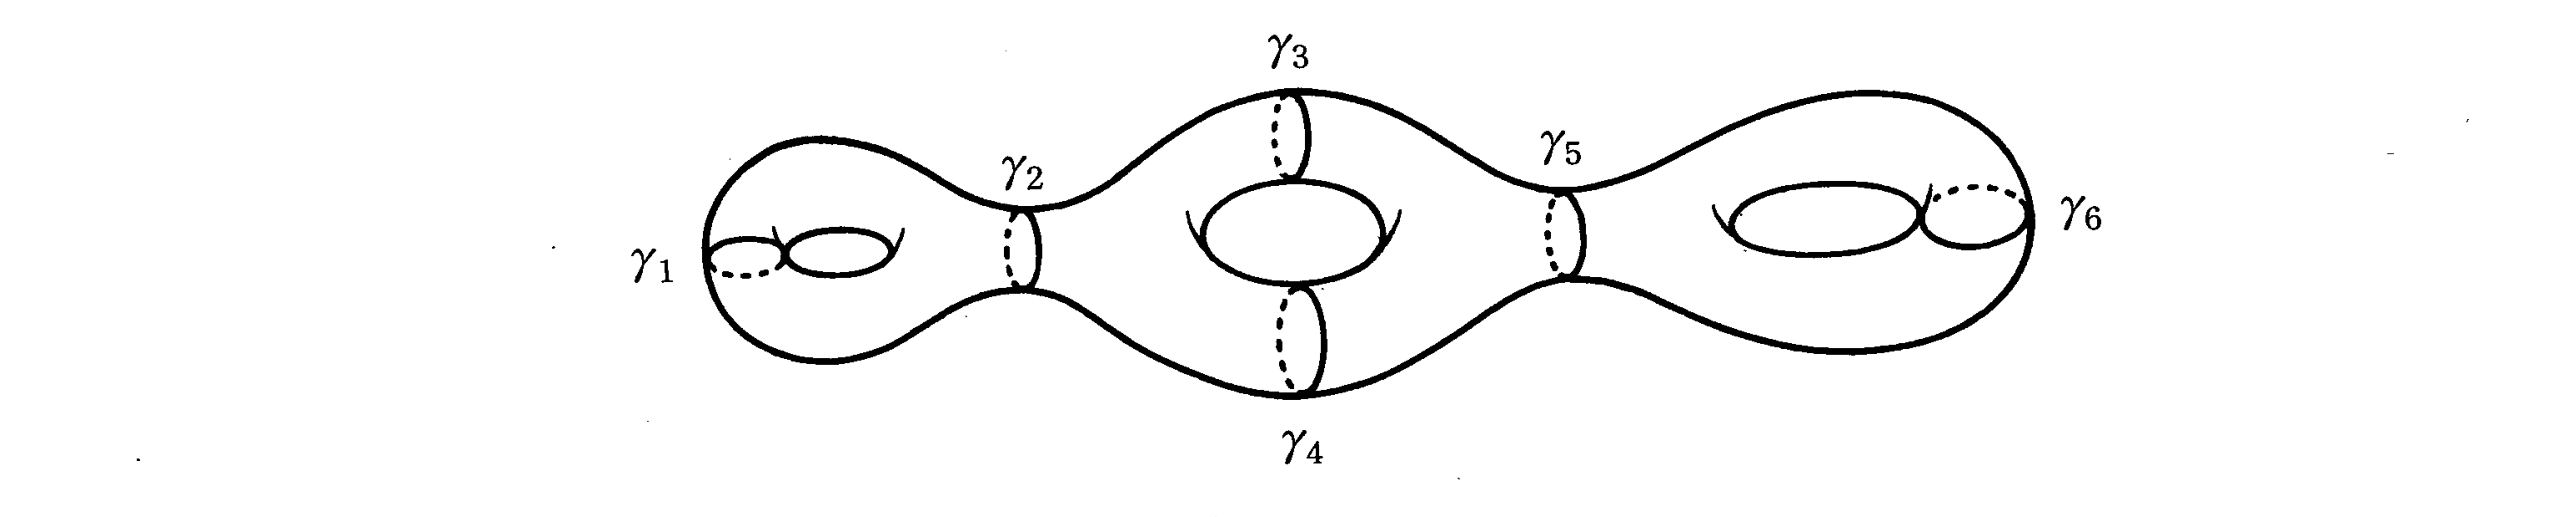
\includegraphics[width=0.95\textwidth]{figures/fig4.7.png}
  \figtitle{4.7}{裤子分解（$g=3$）（原书 p.162）}
\end{figure}

\begin{theorem}{4.117}
  $f$ 的纤维是拉格朗日子流形。
\end{theorem}

\begin{remark}{4.118}
  $R(\Sigma,E)$ 一般有奇点。此外，$f$ 的纤维也可能有奇点。因此，定理只在奇点之外有意义。
\end{remark}

定理 4.117 是下述定理 4.119 的推论。设 $\gamma,\gamma'\in\pi_1(\Sigma)$，置 $f_\gamma([a])=\operatorname{Tr}\operatorname{hol}_a(\gamma)$，$f_{\gamma'}([a])=\operatorname{Tr}\operatorname{hol}_a(\gamma')$。

\begin{theorem}{4.119}
  （Goldman [151]，日文解说见 [211]）
  \[
    \{f_\gamma,f_{\gamma'}\}=\sum_{p\in\gamma\cap\gamma'}\left(f_{\gamma\sharp_p\gamma'}-f_{\gamma\sharp_p\gamma'^{-1}}-f_\gamma f_{\gamma'}\right)
  \]。
  这里 $\gamma\sharp_p\gamma'$ 指把 $\gamma$ 与 $\gamma'$ 在 $p$ 处接起来所得的闭曲线。
\end{theorem}

定理 4.119 的证明省略。

\begin{proof}[定理 4.117 的证明]
  由定理 4.119，$\{f_i,f_j\}=0$。于是由 (4.13)，每个 $f_i$ 在 $f$ 的纤维上为常数，故哈密顿向量场 $V_{f_i}$ 与 $f$ 的纤维相切。因此，在纤维上非奇点的点处，这些向量场张成纤维的切空间。另一方面，由 (4.13) 与 $\{f_i,f_j\}=0$，$\omega(V_{f_i},V_{f_j})=0$。纤维的维数是 $\dim R(\Sigma,E)$ 的一半，故纤维是拉格朗日子流形。
\end{proof}
% [Tutor Note: 这里用的是 Goldman 括号积公式，左端 $\{f_\gamma,f_{\gamma'}\}$ 是 $R(\Sigma,E)$ 上辛结构对应的泊松括号；右端求和遍历 $\gamma$ 与 $\gamma'$ 的横截交点 $p$。图中 $\gamma\sharp_p\gamma'$ 表示先在 $p$ 处沿 $\gamma$ 走一圈再沿 $\gamma'$ 走一圈所得的闭曲线。]

% CHUNK ch04b DONE
